% This is "sig-alternate.tex" V2.1 April 2013
% This file should be compiled with V2.5 of "sig-alternate.cls" May 2012
%
% This example file demonstrates the use of the 'sig-alternate.cls'
% V2.5 LaTeX2e document class file. It is for those submitting
% articles to ACM Conference Proceedings WHO DO NOT WISH TO
% STRICTLY ADHERE TO THE SIGS (PUBS-BOARD-ENDORSED) STYLE.
% The 'sig-alternate.cls' file will produce a similar-looking,
% albeit, 'tighter' paper resulting in, invariably, fewer pages.
%
% ----------------------------------------------------------------------------------------------------------------
% This .tex file (and associated .cls V2.5) produces:
%       1) The Permission Statement
%       2) The Conference (location) Info information
%       3) The Copyright Line with ACM data
%       4) NO page numbers
%
% as against the acm_proc_article-sp.cls file which
% DOES NOT produce 1) thru' 3) above.
%
% Using 'sig-alternate.cls' you have control, however, from within
% the source .tex file, over both the CopyrightYear
% (defaulted to 200X) and the ACM Copyright Data
% (defaulted to X-XXXXX-XX-X/XX/XX).
% e.g.
% \CopyrightYear{2007} will cause 2007 to appear in the copyright line.
% \crdata{0-12345-67-8/90/12} will cause 0-12345-67-8/90/12 to appear in the copyright line.
%
% ---------------------------------------------------------------------------------------------------------------
% This .tex source is an example which *does* use
% the .bib file (from which the .bbl file % is produced).
% REMEMBER HOWEVER: After having produced the .bbl file,
% and prior to final submission, you *NEED* to 'insert'
% your .bbl file into your source .tex file so as to provide
% ONE 'self-contained' source file.
%
% ================= IF YOU HAVE QUESTIONS =======================
% Questions regarding the SIGS styles, SIGS policies and
% procedures, Conferences etc. should be sent to
% Adrienne Griscti (griscti@acm.org)
%
% Technical questions _only_ to
% Gerald Murray (murray@hq.acm.org)
% ===============================================================
%
% For tracking purposes - this is V2.0 - May 2012

\documentclass{sig-alternate-05-2015}


\begin{document}

% Copyright
\setcopyright{acmcopyright}
%\setcopyright{acmlicensed}
%\setcopyright{rightsretained}
%\setcopyright{usgov}
%\setcopyright{usgovmixed}
%\setcopyright{cagov}
%\setcopyright{cagovmixed}

\clubpenalty=10000
\widowpenalty = 10000


%Conference
\conferenceinfo{GECCO'16,} {July 20-24, 2016, Denver, Colorado, USA.}

% \acmPrice{\$15.00}

%
% --- Author Metadata here ---
\CopyrightYear{2016} % Allows default copyright year (20XX) to be over-ridden - IF NEED BE.
\crdata{TBA}  % Allows default copyright data (0-89791-88-6/97/05) to be over-ridden - IF NEED BE.
% --- End of Author Metadata ---

\title{Parent Selection and Diversification}

%
% You need the command \numberofauthors to handle the 'placement
% and alignment' of the authors beneath the title.
%
% For aesthetic reasons, we recommend 'three authors at a time'
% i.e. three 'name/affiliation blocks' be placed beneath the title.
%
% NOTE: You are NOT restricted in how many 'rows' of
% "name/affiliations" may appear. We just ask that you restrict
% the number of 'columns' to three.
%
% Because of the available 'opening page real-estate'
% we ask you to refrain from putting more than six authors
% (two rows with three columns) beneath the article title.
% More than six makes the first-page appear very cluttered indeed.
%
% Use the \alignauthor commands to handle the names
% and affiliations for an 'aesthetic maximum' of six authors.
% Add names, affiliations, addresses for
% the seventh etc. author(s) as the argument for the
% \additionalauthors command.
% These 'additional authors' will be output/set for you
% without further effort on your part as the last section in
% the body of your article BEFORE References or any Appendices.

\numberofauthors{3} %  in this sample file, there are a *total*
% of EIGHT authors. SIX appear on the 'first-page' (for formatting
% reasons) and the remaining two appear in the \additionalauthors section.
%
\author{
% 1st. author
\alignauthor
Thomas Helmuth\\
       \affaddr{Washington and Lee Univ}\\
       \affaddr{Someplace nice}\\
       \affaddr{A city, Virginia}\\
       \email{helmutht@wlu.edu}
% 2nd. author
\alignauthor
Nicholas Freitag McPhee\\
       \affaddr{Div of Sci and Math}\\
       \affaddr{Univ of MN, Morris}\\
       \affaddr{Morris, MN 56267}\\
       \email{mcphee@morris.umn.edu}
% 3rd. author
\alignauthor Lee Spector\\
       \affaddr{Cognitive Science}\\
       \affaddr{Hampshire College}\\
       \affaddr{Amherst, MA}\\
       \email{lspector@hampshire.edu}
}

\maketitle
\begin{abstract}
More things!
\end{abstract}

%
%  Use this command to print the description
%
\printccsdesc

% We no longer use \terms command
%\terms{Theory}

\keywords{lexicase selection, hyperselection, PushGP, other stuff}

\section{Introduction}
\label{sec:introduction}

I bet we start here!

Lexicase selection \cite{Spector:2012:GECCOcompANEW} is nifty, eh?

\section{Experimental Design}

\section{Results}
\label{sec:results}

SOOOO MANY GRAPHS!

\subsection{Starting with high diversity}
\label{sec:highDiversityResults}

\begin{figure*}
	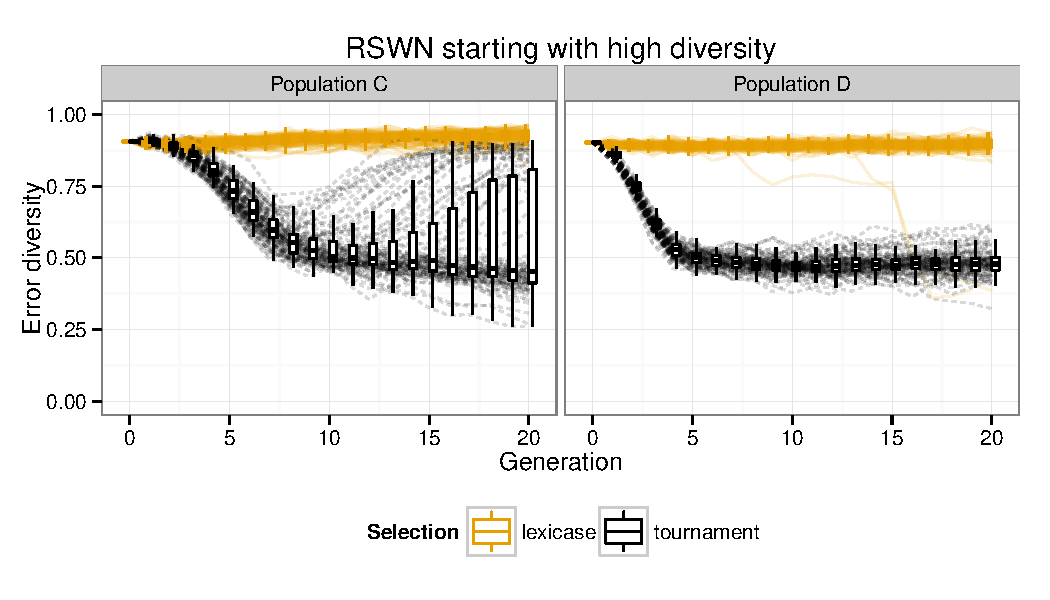
\includegraphics{../figures/RSWN_high_diversity}
	\vspace{-1 cm}
	\caption{Changes in diversity over 100 ``re-runs'' of the replace-space-with-newline problem with both lexicase and tournament selections, starting from a population with high diversity coming from a lexicase selection run.}
	\label{fig:RSWNhighDiversity}
\end{figure*}

\begin{figure*}
	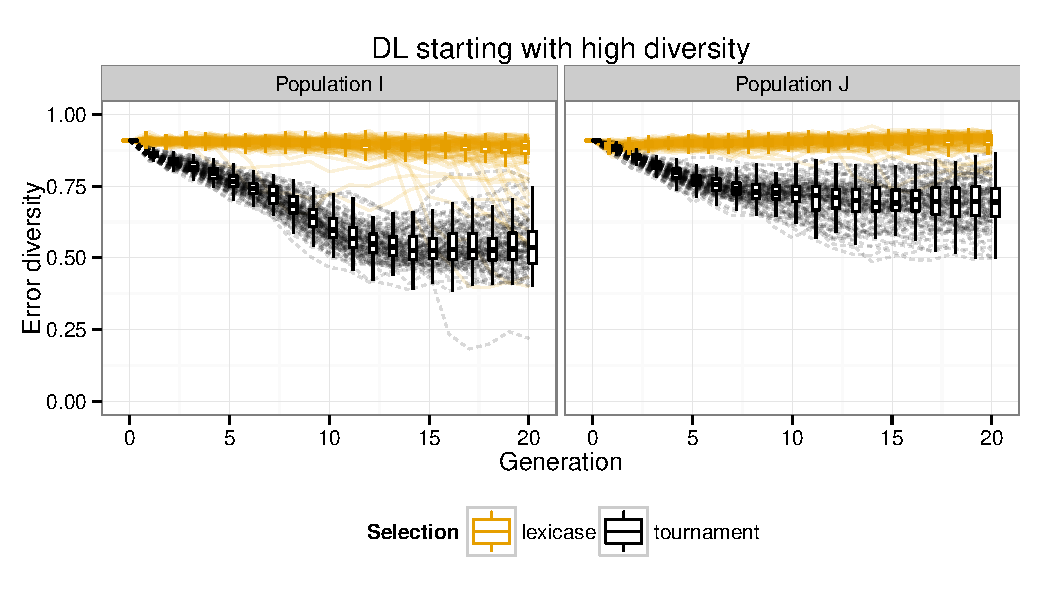
\includegraphics{../figures/DL_high_diversity}
	\vspace{-1 cm}
	\caption{Changes in diversity over 100 ``re-runs'' of the double-letters problem with both lexicase and tournament selections, starting from a population with high diversity coming from a lexicase selection run.}
	\label{fig:DLhighDiversity}
\end{figure*}

\subsection{Starting with low diversity}
\label{sec:lowDiversityResults}

\begin{figure*}
	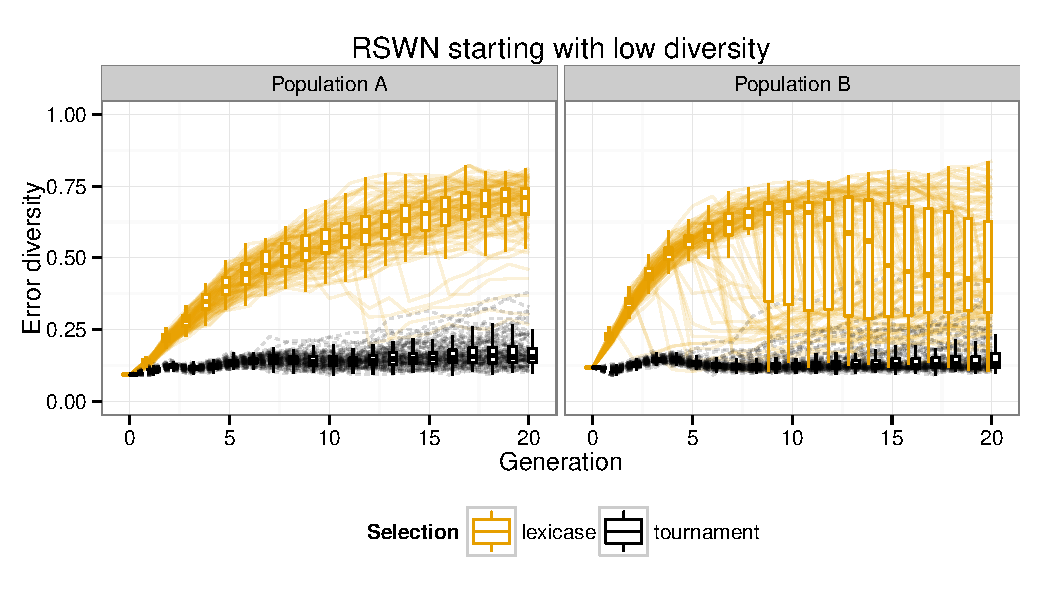
\includegraphics{../figures/RSWN_low_diversity}
	\vspace{-1 cm}
	\caption{Changes in diversity over 100 ``re-runs'' of the replace-space-with-newline problem with both lexicase and tournament selections, starting from a population with low diversity coming from a tournament selection run.}
	\label{fig:RSWNlowDiversity}
\end{figure*}

\begin{figure*}
	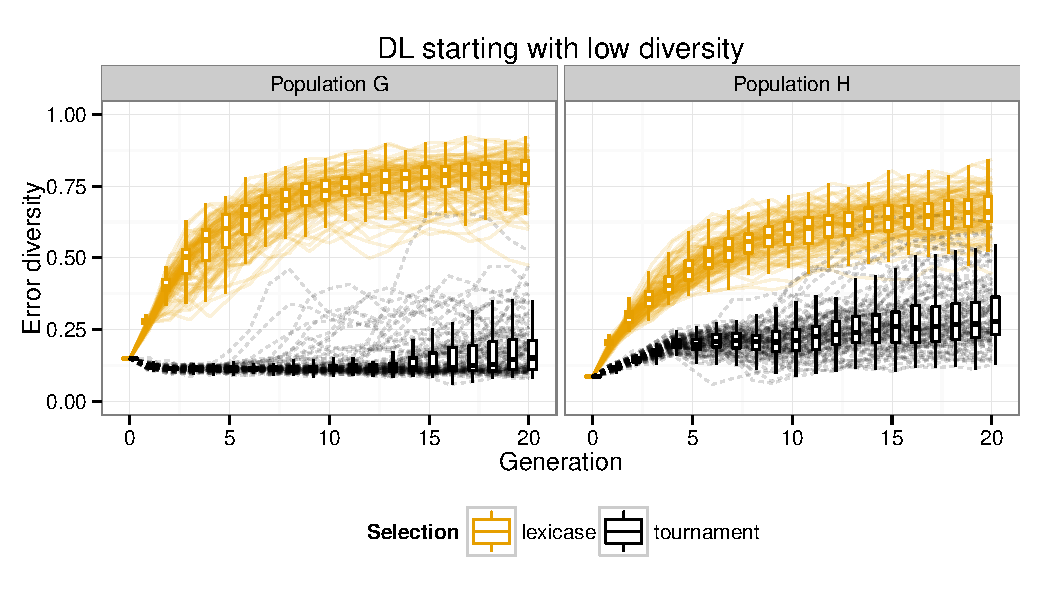
\includegraphics{../figures/DL_low_diversity}
	\vspace{-1 cm}
	\caption{Changes in diversity over 100 ``re-runs'' of the double-letters problem with both lexicase and tournament selections, starting from a population with low diversity coming from a tournament selection run.}
	\label{fig:DLlowDiversity}
\end{figure*}

\subsection{Starting after a diversity crash}
\label{sec:crashDiversityResults}

\begin{figure*}
	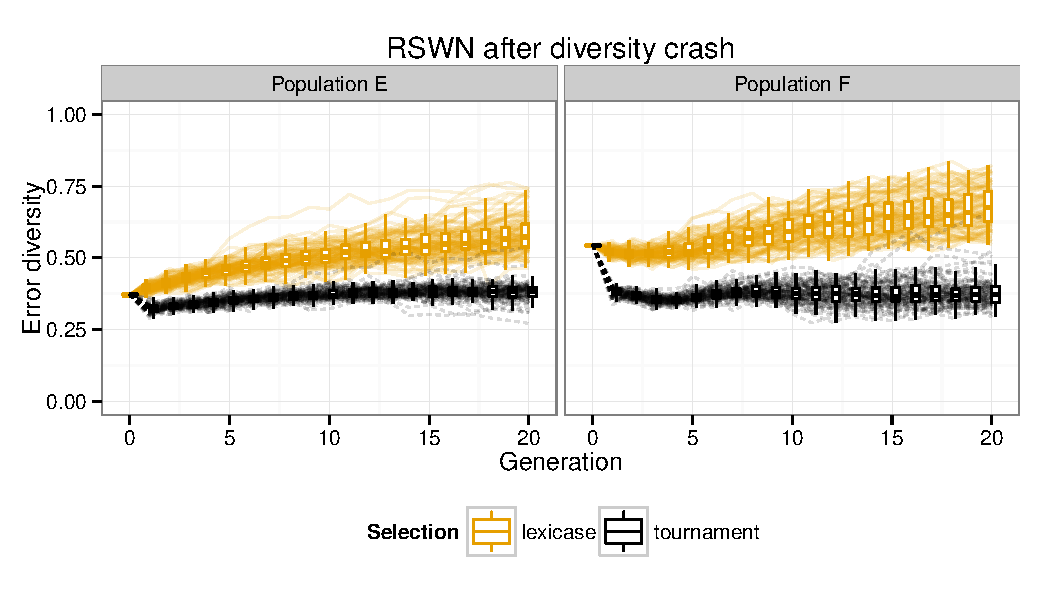
\includegraphics{../figures/RSWN_diversity_crash}
	\vspace{-1 cm}
	\caption{Changes in diversity over 100 ``re-runs'' of the replace-space-with-newline problem with both lexicase and tournament selections, starting from a population with that had lost diversity in a diversity crash in a lexicase selection run.}
	\label{fig:RSWNdiversityCrash}
\end{figure*}

\begin{figure*}
	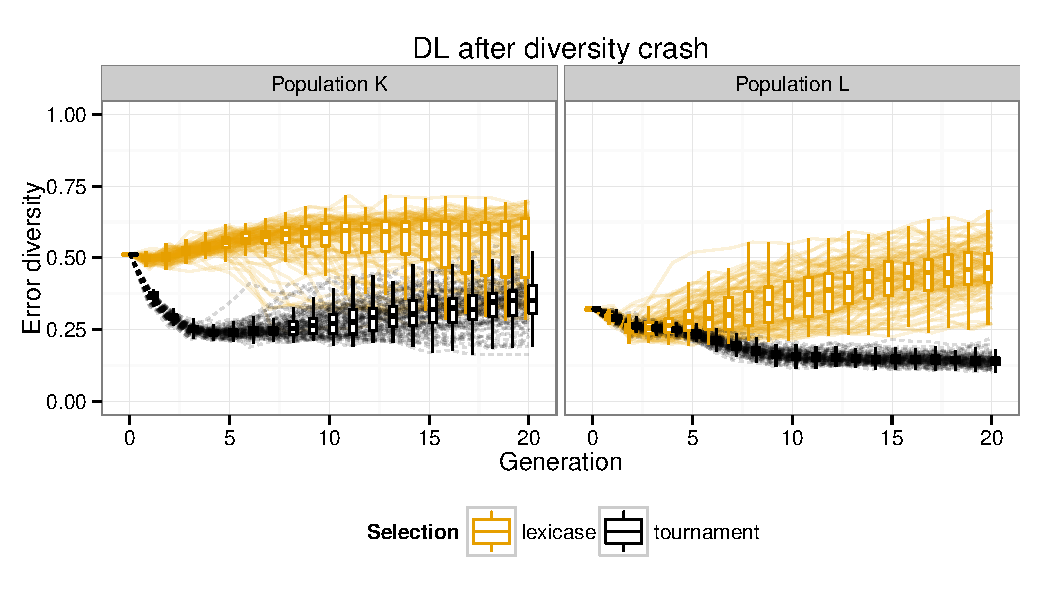
\includegraphics{../figures/DL_diversity_crash}
	\vspace{-1 cm}
	\caption{Changes in diversity over 100 ``re-runs'' of the double-letters problem with both lexicase and tournament selections, starting from a population with that had lost diversity in a diversity crash in a lexicase selection run.}
	\label{fig:DLdiversityCrash}
\end{figure*}

\section{Conclusions}
\label{sec:conclusions}

I'm hoping we have conclusions.

\section*{Acknowledgments}
Lots of cool people helped us.

% The following two commands are all you need in the
% initial runs of your .tex file to
% produce the bibliography for the citations in your paper.
\bibliographystyle{abbrv}
\bibliography{lexicase_recovery}  % sigproc.bib is the name of the Bibliography in this case
% You must have a proper ".bib" file
%  and remember to run:
% latex bibtex latex latex
% to resolve all references
%
% ACM needs 'a single self-contained file'!
%


% \balancecolumns % GM June 2007
\end{document}
